\documentclass[10pt,a4paper]{article}
\usepackage[utf8]{inputenc}
\usepackage[ngerman]{babel}
\usepackage[T1]{fontenc}
\usepackage{amsmath}
\usepackage{amsfonts}
\usepackage{amssymb}
\usepackage{graphicx}
\usepackage{lmodern}
\usepackage{physics}
\usepackage[left=1cm,right=1cm,top=1.5cm,bottom=1.2cm]{geometry}
\usepackage{siunitx}
\usepackage{fancyhdr}
\usepackage{enumerate}
\usepackage{mhchem}
\usepackage{mathtools}
\usepackage{graphicx}
\usepackage{float}
\usepackage{xcolor}
\usepackage{mdframed}
\usepackage{csquotes}
\usepackage{trfsigns}
\usepackage{capt-of}

\sisetup{locale=DE}
\sisetup{per-mode = symbol-or-fraction}
\sisetup{separate-uncertainty=true}
\DeclareSIUnit\year{a}
\DeclareSIUnit\clight{c}
\mdfdefinestyle{exercise}{
	backgroundcolor=black!10,roundcorner=8pt,hidealllines=true,nobreak
}

\begin{document}
\twocolumn
\pagestyle{fancy}
\lhead{DSV Formelsammlung}
\rhead{Sedlmeier, Toni}
\section{Elementare DSV}
%%%%%%%%%%%%%%%%%%%%%%%%%%%%%%%%%%%%%%%%%%%%% Energie %%%%%%%%%%%%%%%%%%%%%%%%%%%%%%%%%%%%%%%%%%%%%%%%%%%%%
  \subsection{Energie}
  Die Leistung und Energie eines Signals $x(k)$ $k \in [k_1,k_2]$
  \begin{mdframed}[style=exercise]
    \begin{align}
        E_{k_1,k_2} &=\sum_{k=k_1}^{k_2} \abs{x(k)}^2 \ = (k_2 - k_1 +1) P_{k_1,k_2} 
    \end{align}
  \end{mdframed}
  Parsevallsche Gleichung ZDFT:
  \begin{mdframed}[style=exercise]
    \begin{align}
        E_{-\infty,\infty} &=\sum_{-\infty}^{\infty} \abs{x(k)}^2 = \frac{1}{2\pi}\displaystyle\int_{-\pi}^{\pi} \abs{X(e^{j\Omega})}^2 d\Omega
    \end{align}
  \end{mdframed}
  Parsevallsche Gleichung DFT:
  \begin{mdframed}[style=exercise]
    \begin{align}
        E &=\sum_{k=0}^{N-1} \abs{x(k)}^2 =\frac{1}{N}\sum_{n=0}^{N-1} \abs{X(n)}^2 
    \end{align}
  \end{mdframed}
  \subsection{DFT/IDFT}
  \begin{mdframed}[style=exercise]
    \begin{align}
        X(n)&=\sum_{k=0}^{N-1} x(k)e^{-j\frac{2\pi kn}{N}} \\
        x(k)&=\frac{1}{N}\sum_{n=0}^{N-1} X(n)e^{-j\frac{2\pi kn}{N}} 
    \end{align}
  \end{mdframed}
%%%%%%%%%%%%%%%%%%%%%%%%%%%%%%%%%%%%%%%%%%%%%%%%%%%%%%%%%%%%%%%%%%%%%%%%%%%%%%%%%%%%%%%%%%%%%%%%%%%%%%%%%%%%%%%
%%%%%%%%%%%%%%%%%%%%%%%%%%%%%%%%%%%%% DFT-Korrespondenzen %%%%%%%%%%%%%%%%%%%%%%%%%%%%%%%%%%%%%%%%%%%%%%%%%%%%%
% Fehler mit scale
\scalebox{0.85}{
    \begin{center}
    \begin{tabular}{ | c | c | c | }
\cline{1-3}
        & Zeitbereich & Spektralbereich \\
\cline{1-3}
        Linearität & $a\cdot x_1(k) b\cdot x_2(k)$ & $a\cdot X_1(n) +b\cdot X_2(n)$ \\
\cline{1-3}
        Zeit-Verschiebung & $x(k\textcolor{red}{-}k_0)$ & $e^{\textcolor{red}{-}j\frac{2\pi nk_0}{N}} X(n)$\\
\cline{1-3}
        Frequenz-Verschiebung & $e^{\textcolor{red}{-}j\frac{2\pi nk_0}{N}} x(k)$ & $X(n\textcolor{red}{+}k_0)$ \\  
\cline{1-3}
        Spiegelung & $x(-k)$ & $X(-n)$ \\  
\cline{1-3}
        Konj.Kompl & $x^*(k)$& $X^*(-n)$\\ 
\cline{1-3}
        Faltung & $x_1(k) \circledast x_2(k)$ & $X_1(n)X_2(n)$ \\  
\cline{1-3}
        Multiplikation & $x_1(k)x_2(k)$ & $\frac{1}{N} X_1(n) \circledast X_2(n)$ \\
\cline{1-3}
        gerade Symmetrie & $x_g(k)=\frac{x(k)+x(-k)}{2}$ & $X_g(n)=\frac{X(n)+X(-n)}{2}$ \\
\cline{1-3}
        ungerade Symmetrie & $x_u(k)=\frac{x(k)-x(-k)}{2}$ & $X_u(n)=\frac{X(n)-X(-n)}{2}$ \\
\cline{1-3}
    \end{tabular}
    \end{center}
}
%%%%%%%%%%%%%%%%%%%%%%%%%%%%%%%%%%%%%%%%%%%%%%%%%%%%%%%%%%%%%%%%%%%%%%%%%%%%%%%%%%%%%%%%%%%%%%%%%%%%%%%%%%%%
%%%%%%%%%%%%%%%%%%%%%%%%%%%%%%%%%%%%% z-Transformation %%%%%%%%%%%%%%%%%%%%%%%%%%%%%%%%%%%%%%%%%%%%%%%%%%%%%
  \subsection{z-Transformation}
  \begin{mdframed}[style=exercise]
    \begin{align}
        X(z) &=\sum_{k=-\infty}^{\infty} x(k)z^{-k} \ \ z=e^{s T_a}
    \end{align}
  \end{mdframed}
%%%%%%%%%%%%%%%%%%%%%%%%%%%%%%%%%%%%%%%%%%%%%%%%%%%%%%%%%%%%%%%%%%%%%%%%%%%%%%%%%%%%%%%%%%%%%%%%%%%%%%%%%%%%
%%%%%%%%%%%%%%%%%%%%%%%%%%%%%%%%%%%%% z-Korrespondenzen %%%%%%%%%%%%%%%%%%%%%%%%%%%%%%%%%%%%%%%%%%%%%%%%%%%%
  \begin{center}
      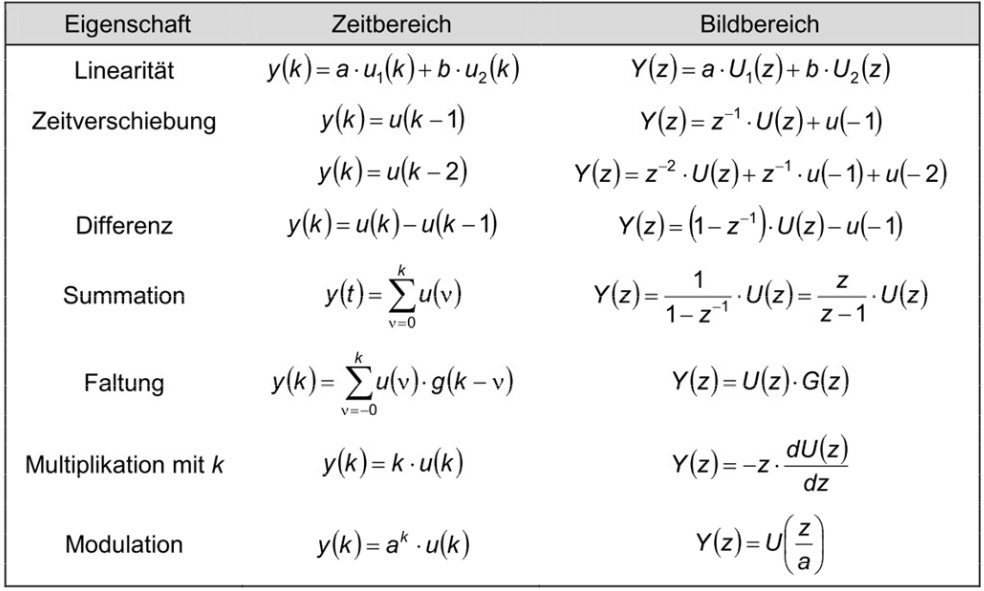
\includegraphics[width=.35\textwidth]{./img/z.png}
  \end{center}
%%%%%%%%%%%%%%%%%%%%%%%%%%%%%%%%%%%%%%%%%%%%%%%%%%%%%%%%%%%%%%%%%%%%%%%%%%%%%%%%%%%%%%%%%%%%%%%%%%%%%%%%%%%%
%%%%%%%%%%%%%%%%%%%%%%%%%%%%%%%%%%%%%%%%%% Faltung %%%%%%%%%%%%%%%%%%%%%%%%%%%%%%%%%%%%%%%%%%%%%%%%%%%%%%%%%
  \subsection{Faltung}
  \subsubsection{Lineare Faltung}
  \begin{mdframed}[style=exercise]
    \begin{align}
        g(k)*u(k) = \sum_{\nu =0}^{k} g(\nu) u(k-\nu)= \sum_{\nu =0}^{k} g(k-\nu) u(\nu)
    \end{align}
  \end{mdframed}
  \subsubsection{Zyklische Faltung}
  $x_1(k)$ und $x_2(k)$ durch \textbf{Zero-Padding} auf $N = N_1 +N_2 -1$ 
  \begin{mdframed}[style=exercise]
    \begin{align}
        x_1(k) \circledast x_2(k) = \sum_{\nu =k_0}^{k_0+N-1} x_1(\nu) x_2(k-\nu)
    \end{align}
  \end{mdframed}
%%%%%%%%%%%%%%%%%%%%%%%%%%%%%%%%%%%%%%%%%%%%%%%%%%%%%%%%%%%%%%%%%%%%%%%%%%%%%%%%%%%%%%%%%%%%%%%%%%%%%%%%%%%%
%%%%%%%%%%%%%%%%%%%%%%%%%%%%%%%%%%%%% Korrelation %%%%%%%%%%%%%%%%%%%%%%%%%%%%%%%%%%%%%%%%%%%%%%%%%%%%%%%%%%
  \subsection{Korrelation}
  $x_1(k) \in [0,N_1-1]$ und $x_2(k) \in [0,N_2-1]$
  \begin{mdframed}[style=exercise]
    \begin{align}
        r_{x1x2}(\lambda) = \sum_{k=-\infty}^{\infty}x_1^*(k) x_2(k+\lambda) 
    \end{align}
  \end{mdframed}
%%%%%%%%%%%%%%%%%%%%%%%%%%%%%%%%%%%%%%%%%%%%%%%%%%%%%%%%%%%%%%%%%%%%%%%%%%%%%%%%%%%%%%%%%%%%%%%%%%%%%%%%%%
%%%%%%%%%%%%%%%%%%%%%%%%%%%%%%%%%%%%% Blocksignalverarbeitung %%%%%%%%%%%%%%%%%%%%%%%%%%%%%%%%%%%%%%%%%%%%
  \subsection{Blocksignalverarbeitung}
  Der $i$-te Block $x^{(i)}(k)$ der Länge $L$ mit Versch.abstand $D$ 
  wird als Multiplikation mit Fensterfunktion $w(k)$ beschrieben
  \begin{mdframed}[style=exercise]
    \begin{align}
        Allg.:
        x^{(i)}(k) = x(k+(i-1)D) \cdot w(k)\ \ k\in[0,L-1] 
    \end{align}
  \end{mdframed}
  Überlapp $D_\%$
  \begin{mdframed}[style=exercise]
    \begin{align}
        D_\% = \frac{L-D}{L}100\%
    \end{align}
  \end{mdframed}
% Overlapp-Add
  \subsubsection{Overlapp-Add Verfahren}
  Schnelle Faltung $g(k)*u(k)$ $N_u >> N_g$ 
  Aufteilung $u(k)$ nicht-überlappend (\textbf{nahtlos}) $\rightarrow D=L$ \\
  Zero-Padding $u^{(i)}(k)$ auf $N=L+N_g$ 
% Overlapp-Save
  \subsubsection{Overlapp-Save Verfahren}
  Schnelle Faltung $g(k)*u(k)$ $N_u >> N_g$ \\
  z.B Überlapp = $N_g-1 \rightarrow D=L-N_g+1$ \\
  \begin{mdframed}[style=exercise]
    \begin{align}
        u^{(i)}(k) = u(k+(i-1)D) \ \ k\in[0,L-1]
    \end{align}
  \end{mdframed}
%%%%%%%%%%%%%%%%%%%%%%%%%%%%%%%%%%%%%%%%%%%%%%%%%%%%%%%%%%%%%%%%%%%%%%%%%%%%%%%%%%%%%%%%%%%%%%%%%%%%%%%%%%
%%%%%%%%%%%%%%%%%%%%%%%%%%%%%%%%%%%%% Simultane Transformation %%%%%%%%%%%%%%%%%%%%%%%%%%%%%%%%%%%%%%%%%%%
  \subsection{Simultane Transformation}
  \begin{mdframed}[style=exercise]
    \begin{align}
        x_1(k) = Re[y(k)] = \frac{1}{2}(y(k)+y^*(k))\\
        x_2(k) = Im[y(k)] = \frac{1}{2j}(y(k)-y^*(k))\\
        x_1(k) = x(2k)\\
        x_2(k) = x(2k+1)\\
        y(k) = x_1(k) +jx_2(k)
    \end{align}
  \end{mdframed}
  \begin{mdframed}[style=exercise]
    \begin{align}
        X_1(n) = \frac{1}{2}(Y(n)+Y^*(-n))\\
        X_2(n) = \frac{1}{2j}(Y(n)-Y^*(n))
    \end{align}
  \end{mdframed}

%%%%%%%%%%%%%%%%%%%%%%%%%%%%%%%%%%%%%%%%%%%%%%%%%%%%%%%%%%%%%%%%%%%%%%%%%%%%%%%%%%%%%%%%%%%%%%%%%%%%%%%%%%
%%%%%%%%%%%%%%%%%%%%%%%%%%%%%%%%%%%%% Stochastische Prozesse %%%%%%%%%%%%%%%%%%%%%%%%%%%%%%%%%%%%%%%%%%%
\section{Stochastische Prozesse}
%%%%%%%%%%%%%%%%%%%%%%%%%%%%%%%%%%%%% Stochastische Variable %%%%%%%%%%%%%%%%%%%%%%%%%%%%%%%%%%%%%%%%%%%
\subsection{Wahrscheinlichkeitsdichtefunktion}
Wahrscheinlickkeit $P(x_u \leq x \leq x_o )$, dass $x \in [x_u,x_o]$ 
  \begin{mdframed}[style=exercise]
    \begin{align}
        P(x_u \leq x \leq x_o ) = \displaystyle\int_{x_u}^{x_o} f_x(\alpha) d\alpha \\
        bzw. \ \ F_x(\alpha) = \displaystyle\int_{-\infty}^{\alpha} f_x(u)du\\
        \displaystyle\int_{-\infty}^{\infty} f_x(u)du = 1
    \end{align}
  \end{mdframed}
Gaußverteilung (Normalverteilung)
  \begin{mdframed}[style=exercise]
    \begin{align}
        f_x(\alpha) = \frac{1}{\sigma_x \cdot \sqrt{2\pi}} \cdot e^{-\frac{1}{2} \cdot \left( \frac{\alpha - \mu_x}{\sigma_x}\right)^2}
    \end{align}
  \end{mdframed}
\subsection{Erwartungswert, Varianz}
  \begin{mdframed}[style=exercise]
    \begin{align}
        \mu_x = E[x] = \displaystyle\int_{-\infty}^{\infty} \alpha f_x(\alpha) d\alpha = \displaystyle\sum_{\nu}^{} a_\nu P_\nu\\
        \sigma_x^2 = E[(x-\mu)^2] = E[x]-\mu^2  = \displaystyle\int_{-\infty}^{\infty} (\alpha-\mu_x)^2 \ f_x(\alpha) d\alpha
    \end{align}
  \end{mdframed}
\subsection{Stationärer Stochastischer Prozess}
P. stationär, wenn seine \textcolor{red}{statistischen} Eigenschaften \textcolor{red}{zeitinvariant} sind \\
Einzelner stationärer Stochastischer Prozess:
  \begin{mdframed}[style=exercise]
    \begin{align}
        f_{x(k)}(\alpha) = f_{x(k+k_0)}(\alpha) = f_x(\alpha)
    \end{align}
  \end{mdframed}
Ein Prozess wird zu zwei verschiedene Zeitpunkte $k_1$ und $k_2$
  \begin{mdframed}[style=exercise]
    \begin{align}
        f_{x(k_1)x(k_2)}(\alpha) = f_{x(k_1+k_0)x(k_2+k_0)}(\alpha)
    \end{align}
  \end{mdframed}
Zwei Prozesse $x$ und $y$ wird zu zwei verschiedene Zeitpunkte $k_1$ und $k_2$
\begin{mdframed}[style=exercise]
    \begin{align}
        f_{x(k_1)y(k_2)}(\alpha) = f_{x(k_1+k_0)y(k_2+k_0)}(\alpha)
    \end{align}
  \end{mdframed}
Autokorrelations $\varphi_{xx}(\lambda)$ und Kreuzkorrelation $\varphi_{xy}(\lambda)$
\begin{mdframed}[style=exercise]
    \begin{align}
        \varphi_{xx}(\lambda) = E[x^*(k)x(k+\lambda)] \\
        \varphi_{xy}(\lambda) =E[x^*(k)y(k+\lambda)]
    \end{align}
  \end{mdframed}
Definition \textbf{schwache Stationarität}
\begin{itemize}
    \item $\mu_x = E[x(k)] = const.$
    \item $\varphi_{xx}(\lambda) = \varphi_{xx}(-\lambda)$ (= gerade Symmetrie)
    \item $\varphi_{xx}(0) \geq \abs{\varphi_{xx}(\lambda)}$ (max(Autokorr.) im Ursprung)
    \item $\varphi_{xx}(0) =E[\abs{x(k)}^2]$ (= mittlere Leistung)
    \item $\varphi_{xx}(0) = \sigma_x^2 + \abs{\mu_x}^2$
\end{itemize}
%%%%%%%%%%%%%%%%%%%%%%%%%%%%%%%%%%%%%%%%%%%%%%%%%%%%%%%%%%%%%%%%%%%%%%%%%%%%%%%%%%%%%%%%%%%%%%%%%%%%%%%%%%
%%%%%%%%%%%%%%%%%%%%%%%%%%%%%%%%%%%%% Ergodizität %%%%%%%%%%%%%%%%%%%%%%%%%%%%%%%%%%%%%%%%%%%
\subsection{Ergodizität}
Scharmittelwert und Zeitmittelwert sind aquivalent\\
\scalebox{0.8}{
    \begin{center}
    \begin{tabular}{|c|c|c|}
\cline{1-3}
        & Zeitmittelwert(Schätzung) & Scharmittelwert \\
\cline{1-3}
        linearer Mittelwert $\mu_x$ & $\mu_x = \frac{1}{N}\sum_{k=0}^{N-1}x(k)$ & E[x(k)] \\
\cline{1-3}
        Varianz $\sigma_x^2$ & $\sigma_x^2 = \frac{1}{N}\sum_{k=0}^{N-1}\abs{x(k)-\mu_x}^2$ & $E[\abs{x(k)-\mu_x}^2]$ \\
\cline{1-3}
        Autokorrelation $\varphi_{xx}(\lambda)$ & $\frac{1}{N}\sum_{k=0}^{N-1} x^*(k)x(k+\lambda) $ & $E[x^*(k)x(k+\lambda)]$ \\
\cline{1-3}
        Kreuzkorrelation $\varphi_{xy}(\lambda)$ & $\varphi_{xy}(\lambda)=\frac{1}{N}\sum_{k=0}^{N-1} x^*(k)y(k+\lambda) $ & $E[x^*(k)y(k+\lambda)]$ \\
\cline{1-3}
    \end{tabular}
    \end{center}
}
%%%%%%%%%%%%%%%%%%%%%%%%%%%%%%%%%%%%%%%%%%%%%%%%%%%%%%%%%%%%%%%%%%%%%%%%%%%%%%%%%%%%%%%%%%%%%%%%%%%%%%%%%%
%%%%%%%%%%%%%%%%%%%%%%%%%%%%%%%%%%%%% Leistungsdichtespektrum %%%%%%%%%%%%%%%%%%%%%%%%%%%%%%%%%%%%%%%%%%%%
\subsection{Leistungsdichtespektrum LDS}
LDS = DFT der Stochastischen Prozesse \\
Autoleistungsdichtespektrum  $\phi_{xx}(e^{j\Omega})$ und Kreuzeistungsdichtespektrum $\phi_{xy}(e^{j\Omega})$
  \begin{mdframed}[style=exercise]
    \begin{align}
        \phi_{xx}(e^{j\Omega}) = \sum_{\lambda=-\infty}^{\infty} \varphi_{xx}(\lambda) e^{-j\Omega\lambda} \\
        \varphi_{xx}(\lambda) = \frac{1}{2\pi} \displaystyle\int_{-\pi}^{\pi} \phi_{xx}(e^{j\Omega})e^{j\Omega\lambda}d\Omega \\
        \phi_{xy}(e^{j\Omega}) = \sum_{\lambda=-\infty}^{\infty} \varphi_{xy}(\lambda) e^{-j\Omega\lambda} \\
        \varphi_{xy}(\lambda) = \frac{1}{2\pi} \displaystyle\int_{-\pi}^{\pi} \phi_{xy}(e^{j\Omega})e^{j\Omega\lambda}d\Omega
    \end{align}
  \end{mdframed}
Mittlere Leistung $\varphi_{xx}(0)$
  \begin{mdframed}[style=exercise]
    \begin{align}
        \varphi_{xx}(0) = \frac{1}{2\pi} \displaystyle\int_{-\pi}^{\pi} \phi_{xx}(e^{j\Omega})d\Omega  = \frac{\phi_{xx}(e^{j\Omega})}{2\pi}
    \end{align}
  \end{mdframed}
Weißes Rauschen (Mittelwertfrei)
  \begin{mdframed}[style=exercise]
    \begin{align}
        \phi_{xx}(e^{j\Omega}) = \phi_0\\
        \varphi_{xx}(0) = \phi_0 \gamma_0(\lambda)
    \end{align}
  \end{mdframed}
%%%%%%%%%%%%%%%%%%%%%%%%%%%%%%%%%%%%%%%%%%%%%%%%%%%%%%%%%%%%%%%%%%%%%%%%%%%%%%%%%%%%%%%%%%%%%%%%%%%%%%%%%%
%%%%%%%%%%%%%%%%%%%%%%%%%%%%%%%%%%%%% LTI-Systeme %%%%%%%%%%%%%%%%%%%%%%%%%%%%%%%%%%%%%%%%%%%%%%%%%%%%%%%%
\subsection{LTI-Systeme}
  \begin{center}
      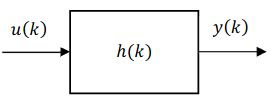
\includegraphics[width=.15\textwidth]{./img/lti.png}
  \end{center}
Mit konst. Mittelwerten $E[u(k-\nu)]=\mu_x$ und $E[y(k)]=\mu_y$
  \begin{mdframed}[style=exercise]
    \begin{align}
        \mu_y = \mu_u \sum_{\nu=-\infty}^{\infty} h(\nu) = \mu_u H(e^{j0})
    \end{align}
  \end{mdframed}
  Zusätzliche Beziehungen
  \begin{mdframed}[style=exercise]
    \begin{align}
        \varphi_{uy}(\lambda) = h(\lambda)*\varphi_{uu}(\lambda) \\
        \varphi_{yu}(\lambda) = h(-\lambda)^**\varphi_{uu}(\lambda) \\
        \varphi_{yy}(\lambda) = h(\lambda)*\varphi_{yu}(\lambda) = h^*(-\lambda)*\varphi_{uy}(\lambda) \\
        \varphi_{yy}(\lambda) = h^*(-\lambda)*h(\lambda)*\varphi_{uu}(\lambda)
    \end{align}
  \end{mdframed}
  \begin{itemize}
      \item $\phi_{uy}(e^{j\Omega}) = H(e^{j\Omega})\phi_{uu}(e^{j\Omega})$
      \item $\phi_{yu}(e^{j\Omega}) = H^*(e^{j\Omega})\phi_{uu}(e^{j\Omega})$
      \item $\phi_{yy}(e^{j\Omega}) = H^*(e^{j\Omega})H(e^{j\Omega})\phi_{uu}(e^{j\Omega}) =\abs{H(e^{j\Omega})}^2 \phi_{uu}(e^{j\Omega}) $ 
  \end{itemize}
%%%%%%%%%%%%%%%%%%%%%%%%%%%%%%%%%%%%%%%%%%%%%%%%%%%%%%%%%%%%%%%%%%%%%%%%%%%%%%%%%%%%%%%%%%%%%%%%%%%%%%%%%%
%%%%%%%%%%%%%%%%%%%%%%%%%%%%%%%%%%%%% Spektralschätzung %%%%%%%%%%%%%%%%%%%%%%%%%%%%%%%%%%%%%%%%%%%%%%%%%%%%%%%%
  \section{Spektralschätzung}
  \subsection{Spektralschätzung mit FFT}
  Umrechnung $n \rightarrow f$
  \begin{mdframed}[style=exercise]
    \begin{align}
        f_n = n\frac{f_A}{N}
    \end{align}
  \end{mdframed}
    \begin{center}
    \begin{tabular}{c c}
        Spektrum & Zeitbereich \\
        $n=0$ & Konstante $x(0)=\frac{1}{N}X(0)$\\
        $n=\tilde{n}$ & $ x_{\tilde{n}}(k)=\frac{1}{N}( X(\tilde{n})e^{-j\frac{2\pi k\tilde{n}}{N}}+X(N-\tilde{n})e^{-j\frac{2\pi k(N-\tilde{n})}{N}})$\\
        $n=\frac{1}{N}$ & $e^{jk\pi} = (-1)^k$\\
    \end{tabular}
    \end{center}
%%%%%%%%%%%%%%%%%%%%%%%%%%%%%%%%%%%%%%%%%%%%%%%%%%%%%%%%%%%%%%%%%%%%%%%%%%%%%%%%%%%%%%%%%%%%%%%%%%%%%%%%%%
%%%%%%%%%%%%%%%%%%%%%%%%%%%%%%%%%%%%% Leck-Effekt %%%%%%%%%%%%%%%%%%%%%%%%%%%%%%%%%%%%%%%%%%%%%%%%%%%%%%%%
\subsection{Leck-Effekt}
Kein Ganzzahliges Vielfaches fällt in das Beobachtungsfenster $w(k)$
  \begin{mdframed}[style=exercise]
    \begin{align}
        x_w(k) = x(k)w(k) \laplace \  X_w(n) = X(n)*W(n) 
    \end{align}
  \end{mdframed}
\end{document}
